% -*- Mode: LaTeX; Package: CLIM-USER -*-

\chapter {Drawing Options}
\label {drawing-options}

This chapter describes the drawing options that are used by CLIM's drawing
functions, and the relationship between drawing options, sheets, and mediums.
These drawing options control various aspects of the drawing process, and can be
provided as keyword arguments to all of the drawing functions.


\section {Medium Components}

Medium objects contain components that correspond to the drawing options; when
no value for a drawing option is explicitly provided to a drawing function, it
is taken from the medium.  These values can be directly queried or modified
using accessors defined on the sheet or medium.  They can also be temporarily
bound within a dynamic context using \cl{with-drawing-options},
\cl{with-text-style}, and related forms.

\cl{setf} of one of these components while it is temporarily bound (via
\cl{with-drawing-options}, for instance) takes effect immediately but is undone
when the dynamic binding context is exited.

In systems that support multiple processes, the consequences are unspecified if
one process reads or writes a medium component that is temporarily bound by
another process.

The following functions read and write components of a medium related to drawing
options.  While these functions are defined for mediums, they can also be called
on sheets support the sheet output protocol and on streams that output to such
sheets.  All classes that support the medium protocol must implement methods for
these generic functions.  Often, a sheet class that supports the output protocol
will implement a ``trampoline'' method that passes the operation on to
\cl{sheet-medium} of the sheet.


\defgeneric {medium-foreground} {medium}
\Defgeneric {medium-background} {medium}

Returns the foreground and background inks (which are designs) for the
\term{medium} \arg{medium}, respectively.  The foreground ink is the default ink
used when drawing.  The background ink is the ink used when erasing.  See
Chapter~\ref{color} for a more complete description of designs.

Any indirect inks are resolved against the foreground and background at the time
a design is rendered.

\defgeneric {(setf medium-foreground)} {design medium}
\Defgeneric {(setf medium-background)} {design medium}

Sets the foreground and background ink, respectively, for the \term{medium}
\arg{medium} to \arg{design}.  You may not set \cl{medium-foreground} or
\cl{medium-background} to an indirect ink.  

\arg{design} is an unbounded design.  If the background design is not completely
opaque at all points, the consequences are unspecified.

Changing the foreground or background of a sheet that supports output recording
causes the contents of the stream's viewport to be erased and redrawn using the
new foreground and background.


\Defgeneric {medium-ink} {medium}

The current drawing ink for the \term{medium} \arg{medium}, which can be any
design.  The drawing functions draw with the color and pattern that this
specifies.  See Chapter~\ref{color} for a more complete description of inks.
The \cl{:ink} drawing option temporarily changes the value of \cl{medium-ink}.

\Defgeneric {(setf medium-ink)} {design medium}

Sets the current drawing ink for the \term{medium} \arg{medium} to \arg{design}.
\arg{design} is as for \cl{medium-foreground}, and may be an indirect ink as
well.


\Defgeneric {medium-transformation} {medium}

The current user transformation for the \term{medium} \arg{medium}.  This
transformation is used to transform the coordinates supplied as arguments to
drawing functions to the coordinate system of the drawing plane.  See
Chapter~\ref{transforms} for a complete description of transformations.  The
\cl{:transformation} drawing option temporarily changes the value of
\cl{medium-transformation}.

\Defgeneric {(setf medium-transformation)} {transformation medium}

Sets the current user transformation for the \term{medium} \arg{medium} to the
\term{transformation} \arg{transformation}.


\Defgeneric {medium-clipping-region} {medium}

The current clipping region for the \term{medium} \arg{medium}.  The drawing
functions do not affect the drawing plane outside this region.  The
\cl{:clipping-region} drawing option temporarily changes the value of
\cl{medium-clipping-region}.

The clipping region is expressed in user coordinates.

\Defgeneric {(setf medium-clipping-region)} {region medium}

Sets the current clipping region for the \term{medium} \arg{medium} to
\arg{region}.  \arg{region} must be a subclass of \cl{area}.  Furthermore, some
implementations may signal an error if the clipping region is not a rectangle or
a region set composed entirely of rectangles.


\Defgeneric {medium-line-style} {medium}

The current line style for the \term{medium} \arg{medium}.  The line and arc
drawing functions render according to this line style.  See
Section~\ref{line-styles} for a complete description of line styles.  The
\cl{:line-style} drawing option temporarily changes the value of
\cl{medium-line-style}.

\Defgeneric {(setf medium-line-style)} {line-style medium}

Sets the current line style for the \term{medium} \arg{medium} to the \term{line
style} \arg{line-style}.


\Defgeneric {medium-default-text-style} {medium}

The default text style for the \term{medium} \arg{medium}.
\cl{medium-default-text-style} will return a fully specified text style, unlike
\cl{medium-text-style}, which may return a text style with null components.  Any
text styles that are not fully specified by the time they are used for rendering
are merged against \cl{medium-default-text-style} using \cl{merge-text-styles}.

The default value for \cl{medium-default-text-style} for any medium is
\cl{*default-text-style*}.

See Chapter~\ref{text-styles} for a complete description of text styles.

\Defgeneric {(setf medium-default-text-style)} {text-style medium}

Sets the default text style for the \term{medium} \arg{medium} to the \term{text
style} \arg{text-style}.  \arg{text-style} must be a fully specified text style.

Some CLIM implementations may arrange to erase and redraw the output on an
output recording stream when the default text style of the stream is changed.
Implementations that do this must obey the proper vertical spacing for output
streams, and must reformat tables, graphs, and so forth, as necessary.  Because
of the expense of this operation, CLIM implementations are not required to
support this.


\Defgeneric {medium-text-style} {medium}

The current text style for the \term{medium} \arg{medium}.  The text drawing
functions, including ordinary stream output, render text as directed by this
text style merged against the default text style.  This controls both graphical
text (such as that drawn by \cl{draw-text*}) and stream text (such as that
written by \cl{write-string}).  See Chapter~\ref{text-styles} for a complete
description of text styles.  The \cl{:text-style} drawing option temporarily
changes the value of \cl{medium-text-style}.

\Defgeneric {(setf medium-text-style)} {text-style medium}

Sets the current text style for the \term{medium} \arg{medium} to the \term{text
style} \arg{text-style}.  \arg{text-style} need not be a fully merged text
style.


\Defgeneric {medium-current-text-style} {medium}

The current, fully merged text style for the \term{medium} \arg{medium}.  This
is the text style that will be used when drawing text output, and is the result
of merging \cl{medium-text-style} against \cl{medium-default-text-style}.


\section {Drawing Option Binding Forms}

\Defmacro {with-drawing-options} {(medium \rest drawing-options) \body body}

Binds the state of the \term{medium} designated by \arg{medium} to correspond to
the supplied drawing options, and executes the body with the new drawing options
specified by \arg{drawing-options} in effect.  Each option causes binding of the
corresponding component of the medium for the dynamic extent of the body.  The
drawing functions effectively do a \cl{with-drawing-options} when drawing option
arguments are supplied to them.

\arg{medium} can be a medium, a sheet that supports the sheet output protocol,
or a stream that outputs to such a sheet.  The \arg{medium} argument is not
evaluated, and must be a symbol that is bound to a sheet or medium.  If
\arg{medium} is \cl{t}, \cl{*standard-output*} is used.  \arg{body} may have
zero or more declarations as its first forms.

\cl{with-drawing-options} must be implemented by expanding into a call to
\cl{invoke-with-drawing-options}, supplying a function that executes \arg{body}
as the \arg{continuation} argument to \cl{invoke-with-drawing-options}.  The exact
behavior of this macro is described under \cl{invoke-with-drawing-options}.

\Defgeneric {invoke-with-drawing-options} {medium continuation \rest drawing-options}

Binds the state of the \term{medium} \arg{medium} to correspond to the supplied
drawing options, and then calls the function \arg{continuation} with the new
drawing options in effect.  \arg{continuation} is a function of one argument,
the medium; it has dynamic extent.  \arg{drawing-options} is a list of
alternating keyword-value pairs, and must have even length.  Each option in
\arg{drawing-options} causes binding of the corresponding component of the
medium for the dynamic extent of the body.

\arg{medium} can be a medium, a sheet that supports the sheet output protocol,
or a stream that outputs to such a sheet.  All classes that obey the medium
protocol must implement a method for \cl{invoke-with-drawing-options}.

The drawing options can be any of the following, plus any of the suboptions for
line styles and text styles.  The default value specified for a drawing option
is the value to which the corresponding component of a medium is normally
initialized.

\Defoption {:ink}

A design that will be used as the ink for drawing operations.  The drawing
functions draw with the color and pattern that this specifies.  The default
value is \cl{+foreground-ink+}.  See Chapter~\ref{color} for a complete
description of inks.

The \cl{:ink} \arg{ink} drawing option temporarily changes the value of
\cl{(medium-ink \arg{medium})} to \arg{ink}, replacing the previous ink; the
new and old inks are not combined in any way.


\Defoption {:transformation}

This transforms the coordinates used as arguments to drawing functions to the
coordinate system of the drawing plane.  The default value is
\cl{+identity-transformation+}.  See Chapter~\ref{transforms} for a complete
description of transformations.

The \cl{:transformation} \arg{xform} drawing option temporarily changes the
value of\cl{(medium-transformation \arg{medium})} to
\cl{(compose-transformations (medium-transformation \arg{medium}) \arg{xform})}.


\Defoption {:clipping-region}

The drawing functions do not affect the drawing plane outside this region.  The
clipping region must be an \cl{area}.  Furthermore, some implementations might
signal an error if the clipping region is not a rectangle or a region set
composed entirely of rectangles.  Rendering is clipped both by this clipping
region and by other clipping regions associated with the mapping from the target
drawing plane to the viewport that displays a portion of the drawing plane.  The
default is \cl{+everywhere+}, or in other words, no clipping occurs in the
drawing plane, only in the viewport.

The \cl{:clipping-region} \arg{region} drawing option temporarily changes the
value of \cl{(medium-clipping-region \arg{medium})} to \cl{(region-intersection
(transform-region (medium-transformation \arg{medium}) \arg{region})
(medium-clipping-region \arg{medium}))}.  If both a clipping region and a
transformation are supplied in the same set of drawing options, the clipping
region argument is transformed by the newly composed transformation before
calling \cl{region-intersection}.

\issue {DCPL} {A better explanation is needed.  It does the right thing, but
it's hard to tell that from this description.  That is, the clipping region is
expressed in user coordinates.}


\Defoption {:line-style}

The line and arc drawing functions render according to this line style.  The
line style suboptions and default are defined in Section~\ref{line-styles}.

The \cl{:line-style} \arg{ls} drawing option temporarily changes the value of
\cl{(medium-line-style \arg{medium})} to \arg{ls}, replacing the previous line
style; the new and old line styles are not combined in any way.

If line style suboptions are supplied, they temporarily change the value of
\cl{(medium-line-style \arg{medium})} to a line style constructed from the
specified suboptions.  Components not specified by suboptions are defaulted from
the \cl{:line-style} drawing option, if it is supplied, or else from the
previous value of \cl{(medium-line-style \arg{medium})}.  That is, if both the
\cl{:line-style} option and line style suboptions are supplied, the suboptions
take precedence over the components of the \cl{:line-style} option.


\Defoption {:text-style}

The text drawing functions, including ordinary stream output, render text as
directed by this text style merged against the default text style.  The default
value has all null components.  See Chapter~\ref{text-styles} for a complete
description of text styles, including the text style suboptions.

The \cl{:text-style} \arg{ts} drawing option temporarily changes the value of
\cl{(medium-text-style \arg{medium})} to \cl{(merge-text-styles \arg{ts}
(medium-text-style \arg{medium}))}.

If text style suboptions are supplied, they temporarily change the value of
\cl{(medium-text-style \arg{medium})} to a text style constructed from the
specified suboptions, merged with the \cl{:text-style} drawing option if it is
specified, and then merged with the previous value of \cl{(medium-text-style
\arg{medium})}.  That is, if both the \cl{:text-style} option and text style
suboptions are supplied, the suboptions take precedence over the components of
the \cl{:text-style} option.


\subsection {Transformation ``Convenience'' Forms}

The following three functions are no different than using
\cl{with-drawing-options} with the \cl{:transformation} keyword argument
supplied.  However, they are sufficiently useful that they are provided as a
convenience to programmers.

In order to preserve referential transparency, these three forms apply the
translation, rotation, or scaling transformation first, then the rest of the
transformation from \cl{(medium-transformation \arg{medium})}.  That is, the
following two forms would return the same transformation (assuming that the
medium's transformation in the second example is the identity transformation):

\begin{verbatim}
(compose-transformations
  (make-translation-transformation dx dy)
  (make-rotation-transformation angle))

(with-translation (medium dx dy)
  (with-rotation (medium angle)
    (medium-transformation medium)))
\end{verbatim}

\Defmacro {with-translation} {(medium dx dy) \body body}

Establishes a translation on the \term{medium} designated by \arg{medium} that
translates by \arg{dx} in the $x$ direction and \arg{dy} in the $y$ direction,
and then executes \arg{body} with that transformation in effect.

\arg{dx} and \arg{dy} are as for \cl{make-translation-transformation}.

The \arg{medium} argument is not evaluated, and must be a symbol that is bound
to a sheet or medium.  If \arg{medium} is \cl{t}, \cl{*standard-output*} is
used.  \arg{body} may have zero or more declarations as its first forms.

\Defmacro {with-scaling} {(medium sx \optional sy origin) \body body}

Establishes a scaling transformation on the \term{medium} designated by
\arg{medium} that scales by \arg{sx} in the $x$ direction and \arg{sy} in the
$y$ direction, and then executes \arg{body} with that transformation in effect.
If \arg{sy} is not supplied, it defaults to \arg{sx}.  If \arg{origin} is
supplied, the scaling is about that point; if it is not supplied, it defaults to
$(0,0)$.

\arg{sx} and \arg{sy} are as for \cl{make-scaling-transformation}.

The \arg{medium} argument is not evaluated, and must be a symbol that is bound
to a sheet or medium.  If \arg{medium} is \cl{t}, \cl{*standard-output*} is
used.  \arg{body} may have zero or more declarations as its first forms.

\Defmacro {with-rotation} {(medium angle \optional origin) \body body}

Establishes a rotation on the \term{medium} designated by \arg{medium} that
rotates by \arg{angle}, and then executes \arg{body} with that transformation in
effect.  If \arg{origin} is supplied, the rotation is about that point; if it is
not supplied, it defaults to $(0,0)$.

\arg{angle} and \arg{origin} are as for \cl{make-rotation-transformation}.

The \arg{medium} argument is not evaluated, and must be a symbol that is bound
to a sheet or medium.  If \arg{medium} is \cl{t}, \cl{*standard-output*} is
used.  \arg{body} may have zero or more declarations as its first forms.

\Defmacro {with-identity-transformation} {(medium) \body body}

Establishes the identity transformation on the \term{medium} designated
by \arg{medium}.

The \arg{medium} argument is not evaluated, and must be a symbol that is bound
to a sheet or medium.  If \arg{medium} is \cl{t}, \cl{*standard-output*} is
used.  \arg{body} may have zero or more declarations as its first forms.



\subsection {Establishing Local Coordinate Systems}

\Defmacro {with-local-coordinates} {(medium \optional x y) \body body}

Binds the dynamic environment to establish a local coordinate system on the
\term{medium} designated by \arg{medium} with the origin of the new coordinate
system at the position $(x,y)$.  The ``directionality'' of the coordinate system
is otherwise unchanged.  \arg{x} and \arg{y} are real numbers, and both default
to 0.

The \arg{medium} argument is not evaluated, and must be a symbol that is bound
to a sheet or medium.  If \arg{medium} is \cl{t}, \cl{*standard-output*} is
used.  \arg{body} may have zero or more declarations as its first forms.

\Defmacro {with-first-quadrant-coordinates} {(medium \optional x y) \body body}

Binds the dynamic environment to establish a local coordinate system on the
\term{medium} designated by \arg{medium} with the positive $x$ axis extending to
the right and the positive $y$ axis extending upward, with the origin of the new
coordinate system at the position $(x,y)$.  \arg{x} and \arg{y} are real
numbers, and both default to 0.

The \arg{medium} argument is not evaluated, and must be a symbol that is bound
to a sheet or medium.  If \arg{medium} is \cl{t}, \cl{*standard-output*} is
used.  \arg{body} may have zero or more declarations as its first forms.


\section {Line Styles\label{line-styles}}

A line or other path is a one-dimensional object.  However in order to be
visible, the rendering of a line must occupy some non-zero area on the display
hardware.  A \concept{line style} represents the advice of CLIM to the rendering
substrate on how to perform the rendering.

\Defprotoclass {line-style}

The protocol class for line styles.
\IfYouWantClass {a} {line style} {line-style}

\Defpredicate {line-style-p} {object}

Returns \term{true} if \arg{object} is a \term{line style}, otherwise returns
\term{false}.

\Defclass {standard-line-style}

An instantiable class that implements line styles.  A subclass of
\cl{line-style}.  This is the class that \cl{make-line-style} instantiates.
\Immutable

\Defun {make-line-style} {\key unit thickness joint-shape cap-shape dashes}

Returns an object of class \cl{standard-line-style} with the supplied
characteristics.  The arguments and their default values are described in
Section~\ref{line-style-options}.


\subsection {Line Style Protocol and Line Style Suboptions\label{line-style-options}}

Each of these suboptions has a corresponding reader that can be used to extract
a particular component from a line style.  The generic functions decribed below
comprise the line style protocol; all subclasses of \cl{line-style} must
implement methods for these generic functions.

\defoption {:line-unit}
\Defgeneric {line-style-unit} {line-style}

Gives the unit used for measuring line thickness and dash pattern length for the
line style.  Possible values are \cl{:normal}, \cl{:point}, or \cl{:coordinate}.
The meaning of these options is:

\begin{itemize}
\item \cl{:normal}---thicknesses and lengths are given in a relative measure in
terms of the usual or ``normal'' line thickness.  The normal line thickness is
the thickness of the ``comfortably visible thin line'',
\footnote{In some window systems, the phrase ``thinnest
visible line'' is used.  This is not appropriate for CLIM, which intends to be
device independent.  (For instance, the thinnest visible line on a 400 d.p.i.
laser printer is a function of the user's viewing distance from the paper.)
Another attribute of a ``normal'' line is that its thickness should
approximately match the stroke thickness of ``normal'' text, where again the
exact measurements are the province of the rendering engine, not of CLIM.}
which is a property of the underlying rendering substrate.  This is the default. 

\item \cl{:point}---thicknesses and lengths are given in an absolute measure in
terms of printer's points (approximately $1/72$ of an inch).
\footnote{This measure was chosen so that CLIM implementors who interface CLIM
to an underlying rendering engine (the window system) may legitimately choose to
make it render as 1 pixel on current (1990) display devices.}

\item \cl{:coordinate}---this means that the same units should be used for line
thickness as are used for coordinates.  In this case, the line thickness is
scaled by the medium's current transformation, whereas \cl{:normal} and
\cl{:point} do not scale the line thickness.
\end{itemize}


\defoption {:line-thickness}
\Defgeneric {line-style-thickness} {line-style}

The thickness, in the units indicated by \cl{line-style-unit}, of the lines or
arcs drawn by a drawing function.  The thickness must be a real number.  The
default is 1, which combined with the default unit of \cl{:normal}, means that
the default line drawn is the ``comfortably visible thin line''.

\defoption {:line-joint-shape}
\Defgeneric {line-style-joint-shape} {line-style}

Specifies the shape of joints between segments of unfilled figures.  The
possible shapes are \cl{:miter}, \cl{:bevel}, \cl{:round}, and \cl{:none}; the
default is \cl{:miter}.  Note that the joint shape is implemented by the host
window system, so not all platforms will necessarily fully support it.

\begin{figure}
\centerline{
\includegraphics{line-joint-shapes}}
\caption{Line joint shapes.}
\end{figure}

\defoption {:line-cap-shape}
\Defgeneric {line-style-cap-shape} {line-style}

Specifies the shape for the ends of lines and arcs drawn by a drawing function,
one of \cl{:butt}, :\cl{square}, \cl{:round}, or \cl{:no-end-point}; the default
is \cl{:butt}.  Note that the cap shape is implemented by the host window
system, so not all platforms will necessarily fully support it.

\begin{figure}
\centerline{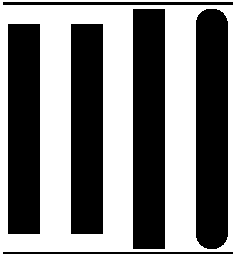
\includegraphics{line-cap-shapes}}
\caption{Line cap shapes.}
\end{figure}

\defoption {:line-dashes}
\Defgeneric {line-style-dashes} {line-style}

Controls whether lines or arcs are drawn as dashed figures, and if so, what the
dashing pattern is.  Possible values are:

\begin{itemize}
\item \cl{nil}---lines are drawn solid, with no dashing.  This is the default.

\item \cl{t}---lines are drawn dashed, with a dash pattern that is unspecified
and may vary with the rendering engine.  This allows the underlying display
substrate to provide a default dashed line for the programmer whose only
requirement is to draw a line that is visually distinguishable from the default
solid line.

\item A sequence---specifies a sequence, usually a vector, controlling the dash
pattern of a drawing function.  It is an error if the sequence does not contain
an even number of elements.  The elements of the sequence are lengths (as real
numbers) of individual components of the dashed line or arc.  The odd elements
specify the length of inked components, the even elements specify the gaps.  All
lengths are expressed in the units described by \cl{line-style-unit}.
\end{itemize}

(See also \cl{make-contrasting-dash-patterns}.)

\subsection {Contrasting Dash Patterns}

\Defun {make-contrasting-dash-patterns} {n \optional k}

If \arg{k} is not supplied, this returns a vector of \arg{n} dash patterns with
recognizably different appearance.  Elements of the vector are guaranteed to be
acceptable values for \cl{:dashes}, and do not include \cl{nil}, but their class
is not otherwise specified.  The vector is a fresh object that may be modified.

If \arg{k} is supplied, it must be an integer between 0 and $\arg{n}-1$
(inclusive), in which case \cl{make-contrasting-dash-patterns} returns the
\arg{k}'th dash-pattern rather than returning a vector of dash-patterns.

If the implementation does not have \arg{n} different contrasting dash patterns,
\cl{make-contrasting-dash-patterns} signals an error.  This will not happen
unless \arg{n} is greater than eight.

\Defgeneric {contrasting-dash-pattern-limit} {port}

Returns the number of contrasting dash patterns that can be rendered on any
medium on the \term{port} \arg{port}.  Implementations are encouraged to make
this as large as possible, but it must be at least 8.  All classes that obey the
port protocol must implement a method for this generic function.
